\chapter{Appendix B: Magic supplementary methods}\label{ch:apd-magic}


\instructionsappendices


\section{Preprocessing: probe to gene mapping}\label{apd:magic-probemap}

A semi-automatic workflow has been developed to consistently annotate probes (Figure \ref{fig:magic-pmap}), i.e. to identify a unique target  gene for each probe whenever possible. In total we needed to map 209036 probes, originating from 27 different microarray platforms. Target genes belong to the “Filtered Gene Set” (FGS) of 5b RefGen v2 B73 maize genome release, since it contains only the high quality gene predictions by removing possible pseudogenes, transposons, contaminations, and low confidence genes. Both the FGS Gene Model and the FGS Transcript Model are used in our workflow, in order to achieve the highest possible mapping coverage for assigning probes to their proper target genes. The Gene Model contains full gene sequences, including exons, introns, 3\textquotesingle\,UTRs, etc, while the Transcript Model  contains only transcript sequences, including splice variants. The workflow consists of four major steps, as is illustrated in Figure \ref{fig:magic-pmap}. First, the collected probe sequences are BLASTed against both the gene model and transcript model. Next, one-to-one probe mappings are extracted by taking all unique hits and identifying the top- hits from multiple hits. The corresponding quality scores are calculated. In the third step, results from the Gene Model BLAST and Transcript Model BLAST are merged into a consistent probe to gene map by resolving possible conflicts between one probe’s gene hit and transcript hit based on the comparison of their quality scores. At last, the mappings retained in previous step are subjected to an additional filtering step to remove low quality hits. Note that we only do quality filtering in the final step in order to maximize the information retained to identify and resolve the potential ambiguous probe sequences. The results are a high quality one-to-one probe to gene mapping.


The results of the workflow are influenced by the characteristics of the input probe sequences, which serve as BLAST query sequences in step 1. We make a distinction between oligo and cDNA probes (respectively 158694 and 60345 in total),. Oligo probe sequences are short sequences of length less than 100 nucleotides, usually sifted through a stringent selection process \cite{Leparc2009,Rouillard2003}.  In contrast, cDNA sequences (which we retrieved from NCBI GenBank based on the access id referred by each probe in the platform specifications), are much longer sequences with length varying between one hundred to several thousand bases. Often generated as a single-pass read, they are of varying quality, and some contain low complexity regions in their sequence. The differences between these two groups are reflected by the parameters used when applying our workflow on them. In the initial BLAST step, an $e$-value cutoff $0.001$ is used for oligo due to their shorter length. In contrast, a much stricter $e$-value cutoff 1e-20 is applied for cDNA to avoid hits over low quality regions and to compensate their longer sequence length. Conversely, a stricter criterion for oligos is employed to guarantee the mapping quality in the final filtering step, as even small variances between probe and target sequences can have a great influence on their binding specificity due to the short sequence length. A looser criterion is utilized for cDNA assuming that longer probe sequences can tolerate more sequence variation and still bind the proper target transcripts.

In the next sections, the individual steps of the workflow, and the results obtained from each step, will be discussed in greater detail.

\begin{figure}
	\centering
	\medskip
  	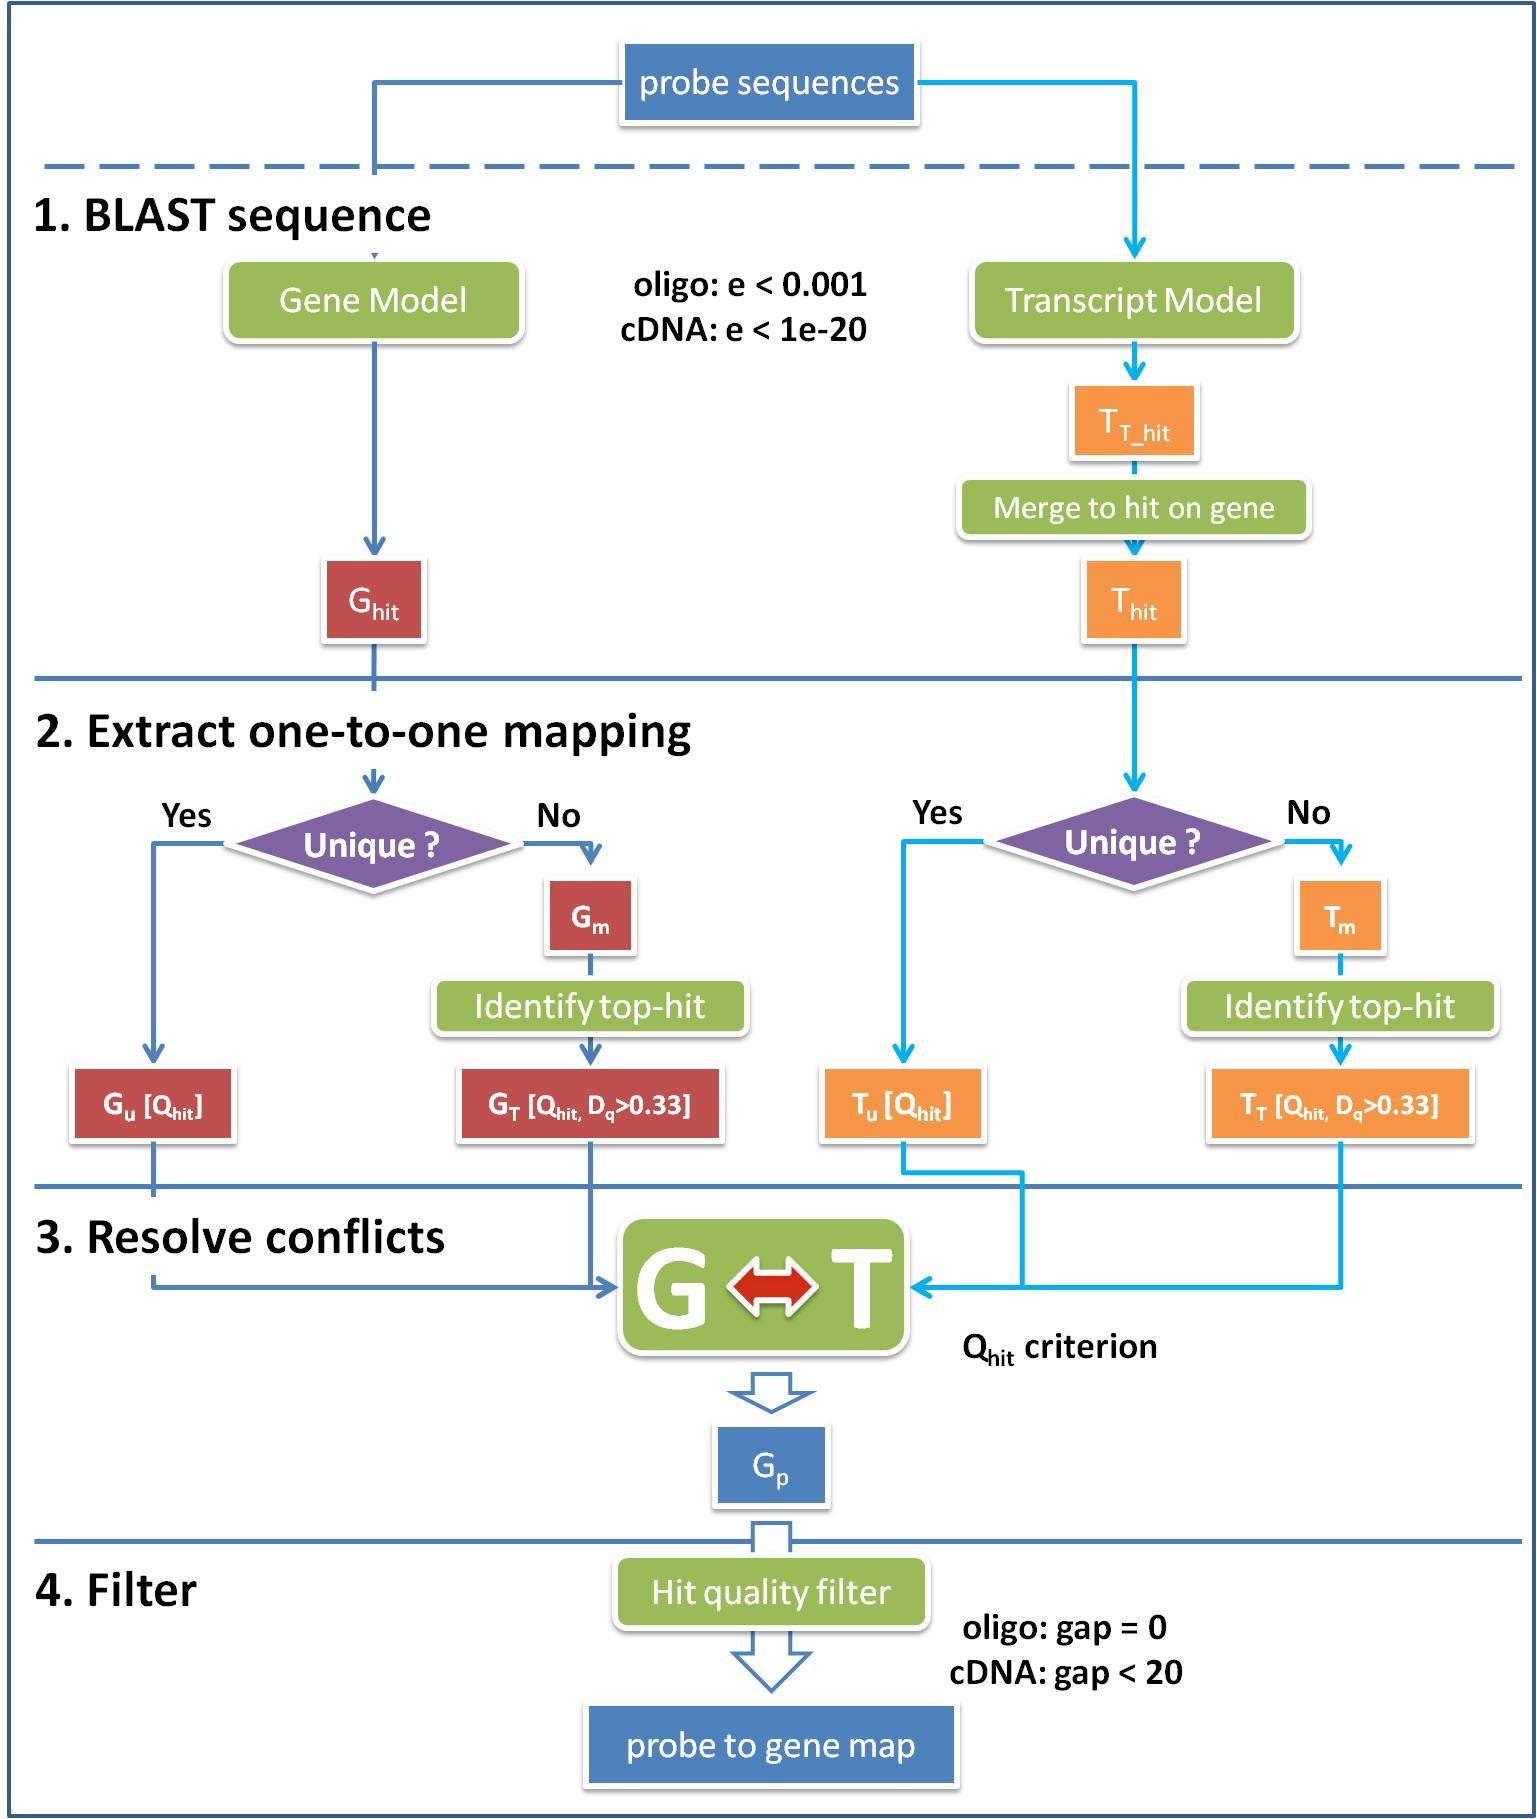
\includegraphics[width=1\textwidth]{ApdxB-workflow.jpg}
  	\caption[Probe to gene mapping workflow]
  	{Probe to gene mapping workflow. The workflow consists of four
  	steps. First, the probe sequences collected are BLASTed against
  	both the FGS Gene and Transcript Model. Next, one-to-one probe
  	mappings are extracted by taking all unique hits ($G_u$, $T_u$) and
  	identifying top-hits ($G_T$,$T_T$) from multiple hits ($G_m$,$T_m$). For all
  	hits the quality measurements $Q_{hit}$ and $D_q$ are calculated. In the
  	third step, results from Gene Model BLAST and Transcript Model
  	BLAST are merged into a consistent probe to gene map ($G_p$) by
  	resolving possible conflicts between one probe’s gene hit and
  	transcript hit using $Q_{hit}$. At last, $G_p$ is filtered to remove low
  	quality hits, resulting in a high quality one-to-one probe to
  	gene mapping.}
  	\label{fig:magic-pmap}
\end{figure}


\begin{table}
	\centering
	\begin{threeparttable}
	\begin{footnotesize}
	\caption{Probe mapping for cDNA and oligo probes for \textit{Zea mays}}
	\label{tab:magic-probemap}
	\begin{tabular}{@{}p{3cm}r|rcr|r}
	\toprule

	& \multicolumn{2}{c}{\textbf{cDNA}} & \phantom{a} & 
	\multicolumn{2}{c}{\textbf{Oligo}} \\
	
	\cmidrule{2-3} \cmidrule{5-6}
	
	& & \textbf{Transcript}	&& & \textbf{Transcript} \\
	& \textbf{Gene blast} & \textbf{blast} && \textbf{Gene blast}	& 
	\textbf{blast} \\
	
	\midrule
	
	{\it ~~~Probe total\tnote{2}} & \multicolumn{2}{r}{60345} &&	
			\multicolumn{2}{r}{158694} \\[1.5ex]

		\multicolumn{6}{l}{Step 1 - Mapping with megablast} \\[.2ex]
	{\it ~~~Hits total\tnote{3}} & 153050 & 130927 && 129097 & 123089 \\
	{\it ~~~Hit transcripts\tnote{4}} & - & 42250 && - & 49289 \\
	{\it ~~~Hit genes\tnote{5}} & 24495 & 23393 && 28879 & 
	28416 \\
	{\it ~~~Probes retained} & 57700 & 56852 && 99139 & 105429 \\
	
	\multicolumn{6}{l}{}\\
		
		\multicolumn{6}{l}{Step 2 - Extracting one-to-one mappings} 
		\\[.2ex]
	{\it ~~~Unique hits\tnote{6}} & 24766 & 24820 && 84854 & 92878 \\
	\multicolumn{6}{l}{{\it ~Multiple hits}} \\
	{\it ~~~~~Hits count\tnote{3}} & 128284 & 106107 && 44243 & 30211 \\
	{\it ~~~~~Probe count} & 32934 & 32032 && 14285 & 12551 \\
	{\it ~~~~~Top hits\tnote{7}} & 9067 (27.5\%) & 12979 (40.5\%) && 11 (0.0\%) 
	& 11 (0.0\%)\\
	
	\multicolumn{6}{l}{}\\
				
		\multicolumn{6}{l}{Step 3 - Merging blast results\tnote{8}} \\[.2ex]
	{\it ~~~Unique maps\tnote{9}} & 898 & 40 && 7697 & 13987 \\
	{\it ~~~Identical maps\tnote{10}} & 
			\multicolumn{2}{r}{52084} && \multicolumn{2}{r}{90482} \\
	{\it ~~~Conflicts\tnote{11}} & 
			\multicolumn{2}{r}{2647 (4718)} && \multicolumn{2}{r}{6 (953)} \\
	{\it ~~~Sum\tnote{12}} & 
			\multicolumn{2}{r}{38563 (\textit{57740})} && 
			\multicolumn{2}{r}{97001 (\textit{113119})} \\

	\multicolumn{6}{l}{}\\

		\multicolumn{6}{l}{Step 4 - Filtering by quality} \\[.2ex]
	{\it ~~~Probes removed} & \multicolumn{2}{r}{414} && 
			\multicolumn{2}{r}{6870} \\

	\multicolumn{6}{l}{}\\
		
		\multicolumn{6}{l}{Result} \\[.1ex]
	{\it ~~~~Contribution\tnote{13}} & 4305 (11.3\%) & 33844 && 5187 
			(5.8\%) & 84944 \\
	{\it ~~~Total} & \multicolumn{2}{r}{38149} && 		
			\multicolumn{2}{r}{90131} \\
	\bottomrule
	\end{tabular}
	\end{footnotesize}
	\begin{scriptsize}
	\begin{tablenotes}
	\item[1] If not noted, the number of unique probes of a corresponding 
		category is reported in the table.
	\item[2] The same set of probe sequence is used in both the gene blast and 	
		the transcript blast procedure.
	\item[3] The number of BLAST hits of a corresponding category is reported.
	\item[4] $T_{T\_hit}$, the number of unique transcripts having at least one 
		hit is reported.
	\item[5] The number of unique genes having at least one hit is reported.
	\item[6] For unique hits where a probe hits only on one target 
		(gene/transcript), these three numbers are equal, the number of hits, 
		the number of unique targets, and the number of the unique probes.
	\item[7] The number of probes and the corresponding percentages that the 
		top hits pass $D_q$ criterion.
	\item[8] In this step, the hits from different blasts are merged to form 
		one-to-one probe to gene mappings. To contrast the results with those
		obtained in previous steps, each record in them are called a 
		\textit{map} instead of a \textit{hit} in the later steps.
	\item[9] Probes whose targets are only identified by one blast procedure.  
		Further breakdowns of the data based on hit type are available in Table 
		\ref{tab:magic-uniquemaps}.
	\item[10] Probes for which both gene blast and transcript blast identify the
	 	same targets.  Further breakdowns of the data into different 
	 	categories are available in Table \ref{tab:magic-map-comparison}.
	\item[11] Probes for which different targets are identified by gene blast 
		and transcript blast (a conflict), showing the number of resolved 
		conflicts with the total number of conflicts between brackets. Please 
		check Section \ref{apd:magic-conflict} for details, and a data 
		breakdown in Table \ref{tab:magic-map-comparison}.
	\item[12] The total number of probes left in the final merged mappings. In 
		bracket, the raw total count before removing ambiguous top hits.
	\item[13] The number of probes obtaining maps from each blast analysis.
	\end{tablenotes}
	\end{scriptsize}
	\end{threeparttable}
\end{table}



\subsection{Step 1 – Mapping with megablast}

First, the probe sequences (BLAST queries) are blasted against both the gene model and transcript model (BLAST targets) using megablast version 2.2.17  (\cite{Zhang2000}).  BLAST on both the FGS Gene Model and Transcript Model was done to recover as much of the tentative targets of each probe, because the collected probe sequences, especially the cDNA ones, sometimes contain also introns.   In addition, for certain sequences, BLAST on the transcript model alone will result in poor quality hits, and as a consequence, for many probes  no target gene can be identified.  To retain as much information as possible from the blast results we choose a relative loose criterion to BLAST sequences.  Except for the different $e$-value cutoffs, the common parameters applied for both cDNA sequences and oligo sequences are ‘$-F\:F$’ to turn off the query sequence filtering, ‘$-b\:15$’ to list only the top 15 hits.

BLAST on the Gene Model generates a set of hits $G_{hit}$, each of which maps a probe to a gene; BLAST on the Transcript Model generates a different set of hits $T_{T\_hit}$, which maps a probe to a transcript. $T_{T\_hit}$ are converted into hits on genes in two steps. First, all hits of a probe to a transcript are grouped by the corresponding genes of the hit transcripts. Second, each group of hits is merged into one hit on that gene, while the best transcript hit score in the group is retained as the gene hit score. After this conversion, both Gene Model BLAST results $G_{hit}$  and the Transcript Model BLAST results $T_{hit}$ map probes to gene identifiers. Nevertheless, to distinguish between the gene and transcript hit, we keep referring to the probe-to-gene hits originating from the Transcript Model BLAST ($T_{hit}$) as the probe-to-transcript hits.  

After applying this step, the results obtained are summarized in the Table \ref{tab:magic-probemap} (Step 1). The number of the transcript hits is nearly the double of the number of the gene hits. When mapped to a gene, many probes in each category hit on the different transcripts of a gene (data not shown), indicating that they are not designed to distinguish different transcripts (splice variants) of the same gene.

\subsection{Step 2 – Extracting one-to-one mappings}

In this step, we try to extract one-to-one probe to gene mapping from both the $G_{hit}$ and $T_{hit}$ lists independently. The gene hit and transcript hit results are kept separately to better resolve the possible conflicts between them in the next step. Based on the number of identified target genes a probe sequence has, both $G_{hit}$ and $T_{hit}$ are divided into unique-hit group and multi-hit group, where a single probe maps to only one gene or on several genes respectively. This results in 4 groups: 

\begin{itemize}
\item $G_u$, gene unique-hit
\item $T_u$, transcript unique-hit
\item $G_m$, gene multi-hit
\item $T_m$, transcript multi-hit
\end{itemize}

Next, we calculate a hit quality score $Q_{hit}$ for each hit, based on its BLAST information as follows:  

\begin{equation}
Q_{hit} = coverage * identity - 3 * num\_gaps / query\_length
\end{equation}

in it, \textit{coverage},  \textit{identity}, and \textit{num\_gaps} (number of gaps) are characteristics of the BLAST hit, and $3$ is empirically chosen such that enough penalty is given to gaps but not overweight it so much that $Q_{hit}$ can become negative. As a simple percentage, the score takes into the consideration the percentage of exact match nucleotides on probe sequence and the number of gaps in the match region. Those are important factors that influence probe to target specificity.  \\
We use this scores to resolve the multiple mapping issues in the multi-hit groups ($G_m$ and $T_m$) by identifying a promising best hit for each probe -if possible-. First, all hits of a probe are ranked by their $Q_{hit}$s. The hit with the highest score are kept, resulting in $G_t$, the gene top-hits, and $G_t$, the transcript top-hits.Then, the difference $D_q$ between the scores of the top two hits is calculated. It serves as a proxy for the binding specificity difference between first two hits. When the following condition is met: 

\begin{equation}
D_q = Q_{hit_{1st}} - Q_{hit_{2nd}} \geq 0.33
\end{equation}

the hit with the highest score (top hit) is assumed to be the target of the probe, i.e. considered more likely to bind the probe sequence compared to other hits. If the above condition is not met, the corresponding results for that probe are marked, assuming that they can hybridize several genes and generate ambiguous expression measurements. They are kept temporarily to identify possible conflicts between gene and transcript blast output, and to resolve the conflicts by comparing hits quality. 

The result of this step is summarized in Table \ref{tab:magic-probemap} (Step 2). Clearly, the short oligo probe sequences are much more target specific when compared with the cDNA sequences, with the majority being unique hits and much less multiple mapping probes. In contrast, cDNA probe sequences, although much longer, tend to produce partial hits on several genes, due to the relative loose BLAST settings in the step 1. Filtered by the $D_q$ criterion, the true target gene (top hit) can be identified in many cases ($27.5\%$ of $G_m$ and $40.5\%$ of $T_m$). Whereas for oligo probes, this is rather rare (11 cases in both $G_m$ and $T_m$).


\begin{table}[tb]
	\centering
	\begin{threeparttable}
	\begin{footnotesize}
	\caption{Statistics of unqiuely mapped probes} 
	\label{tab:magic-uniquemaps}
	\begin{tabular}{@{}>{\centering\arraybackslash}p{5cm}rcr}
	\toprule
	 \textbf{Probe blast hit type} & \textbf{cDNA} & \phantom{a} & 
	 \textbf{oligo} \\
	\midrule
	
	\multicolumn{4}{l}{\textit{Gene blast}} \\
	~~$G_u$ & 344 && 5609 \\
	~~$G_t$ & 554 && 2088 \\
	\textit{Sub total} & 898 && 7697 \\[1.5ex]

	\multicolumn{4}{l}{\textit{Transcript blast}} \\
	~~$T_u$ & 40 && 11937 \\
	~~$T_t$ & 10 && 2050 \\
	\textit{Sub total} & 50 && 13987 \\

	\bottomrule
	\end{tabular}
	\end{footnotesize}
	\end{threeparttable}
\end{table}


\begin{table}[t]
	\centering
	\begin{footnotesize}
	\caption{Breakdown of the queries who have hits in both gene and transcript 
		blast} 
	\label{tab:magic-map-comparison}
	\begin{tabular}{@{}>{\centering\arraybackslash}p{1.7cm}
	>{\centering\arraybackslash}p{2cm} rrcrr}
	\toprule

	 &  &  \multicolumn{2}{c}{\textbf{cDNA}} & \phantom{a} & 
	\multicolumn{2}{c}{\textbf{oligo}} \\

	\cmidrule{3-4} \cmidrule{6-7}

	\textbf{Gene hit} & \textbf{Trans. hit} &
	\textbf{Identical} & \textbf{Conflict} 
	&& 
	\textbf{Identical} & \textbf{Conflict}  \\
	
	\midrule
	
	$G_u$ & $T_u$ & 23542 & 0 && 79152 & 7(0) \\
	$G_t$ & $T_t$ & 26788 & 4354 (579, 1885) && 10102 & 313(0) \\
	$G_u$ & $T_t$ & 821 & 59 (4, 17) && 72 & 14(0) \\
	$G_t$ & $T_u$ & 933 & 305 (147, 15) && 1156 & 626(6, 0) \\
	
%	BACKUP, before statistic without 'Mweight_diff >= .33' 
%
%	$G_u$ & $T_u$ & 23542 & 0 && 79152 & 7 \\
%	$G_t$ & $T_t$ & 7070 & 38 (14, 4) && 9 & 0 \\
%	$G_u$ & $T_t$ & 590 & 7 (0, 4) && 0 & 0 \\
%	$G_t$ & $T_u$ & 477 & 39 (39, 0) && 2 & 0 \\

%   BACKUP, data before apply 'Mweight_diff >= .33' to filter tophit
%
%	$G_u$ & $T_T$ & 821 & 59 && 72 & 14 \\
%	$G_T$ & $T_u$ & 933 & 305 && 1156 & 626 \\

	\bottomrule
	\end{tabular}
	\end{footnotesize}
\end{table}



\subsection{Step 3 – Merging blast results}

Till now we have identified one target gene for each probe separately for gene blast analysis and transcript blast analysis. Next we need to combine these two sets into one consistent result set.  There are different cases when combining two data sets. The first case is the `\textit{unique map}', where the result is obtained in only one blast analysis. In this case, the blast data are taken directly into the final data set. When both blast analyses identify the same gene as target, it is the case of `\textit{identical map}'. The genes identified are taken as the target, and the best blast hit raw data are retained for further analysis. At last there is `\textit{conflict}' when two blast analysis identify different genes as the target of a probe.  In this case, an extra step is taken to resolve the conflict by identifying the possibly most reliable target out of the two candidates when possible. If this fails, the probe is discarded from the result set. The detail of the conflict resolving strategy is explained in the next section.

The statistic data of this analytical step is summarized in Table \ref{tab:magic-probemap} (Step 3), showing the probe count for each aforementioned cases. For the conflicts, it shows the probe count for the resolved cases with the total number of conflicts between brackets. Recall that in previous step, we only marked the ambiguous top-hits. Those ambiguous results retained in the merged result sets are removed before the next step. This results a big reduction of the cDNA probes mapped, dropping from 57740 to 38563 (33.2\% less). Whereas for oligo probes, there is a 14.2\% drop, removing 16118 out of 113119 probes. (Table \ref{tab:magic-probemap}).


\subsubsection{Resolving conflicts}\label{apd:magic-conflict}

There is a \textit{conflict} if for one probe, the target gene of the transcript blast hit ($T_u$/$T_t$) are different from that of the gene blast hit ($G_u$/$G_t$). In previous steps, we grouped the results obtained by each blast analysis into two sets, unique hit and top hit. These results in 4 groups in total, $G_u$, $T_u$, $G_t$, and $T_t$.The conflicts among them are resolved according to a set of heuristic rules. Note that by definition, there are no conflicts between the result sets obtained from the same blast results (gene or transcript model), such as ($G_u$, $G_t$) and ($T_u$, $T_t$). For each conflict, the following condition based on $Q_{hit}$ is evaluated: 

\begin{equation}
ABS(Q_{T_{hit}}-Q_{G_{hit}}) \geq 0.2
\end{equation}

when true, the one with the higher $Q_{hit}$ was chosen to be the real target gene; otherwise, the hits of corresponding probe are discarded from the results due to having ambiguous target genes. Note, the $Q_{hit}$ cutoff used here is less strict than the one used in identifying top-hit from multiple mapping probes, since here we compare two potential hits from different BLAST results, while before hits of same BLAST results were compared.

Depending on the sources between which the conflict arises, there are three types of conflicts:

\begin{itemize}
\item Conflicts between a pair of unique-hits, i.e. from ($G_u$, $T_u$). There are no such conflicts for the cDNA hits, and 7 conflicts for the oligo hits. Checking their gene unique hit results, we found that all those hits reside fully or partially in the intron region. Consequently, those genes could not be identified as targets by blast against the transcript model. Similarly, the unique transcript hits are across exon boundaries of hit genes, and as such they do not appear in the gene model blast results. After applying our $Q_{hit}$ criterion, none passed the check and all  were discarded. 

\item  Conflicts between one unique-hit and one top-hit, i.e. between ($G_u$, $T_t$) or ($G_t$, $T_u$). There are many such conflicts for both the cDNA probes and the oligo probes. By applying the above $Q_{hit}$ condition, nearly half of the conflicts can be resolved for the cDNA probes. However, for the oligo probes, this succeeds in only 6 cases (Table \ref{tab:magic-map-comparison}). And the resolved cases are mostly won by the top hits. In the table \ref{tab:magic-conflict-topuniq}, one example is given for each subtype where the conflict is resolved. 

\begin{table}[b]
	\centering
	\begin{footnotesize}
	\caption{The conflicts between a top hit and an unique hit} 
	\label{tab:magic-conflict-topuniq}
	\begin{tabular}{@{}c|cccccc@{}}
	\toprule
	& \textbf{Hit} & & & \textbf{Match} & & \\
	& \textbf{type} & \textbf{Target} & \textbf{Coverage} & \textbf{length} 
	& \textbf{Gaps} & \textbf{$e$-value} \\ 
	\midrule
	& $2^{nd}$  & GRMZM2G020553 & 61.8267 & 250 & 4 & $1.00E-107$ \\ 
	Case 1 & \textbf{$G_t$} & \textbf{GRMZM5G865576} & 94.61358 & 403 & 2 & 0 
	\\ 
	& $T_u$ & GRMZM2G020553 & 61.8267 & 250 & 4 & $1.00E-108$ \\

 	\hline
 	
	& $G_u$ & AC206201.3\_FG004 & 14.61412 & 89 & 0 & 5.00E-43 \\
	Case 2 & $2^{nd}$ & AC206201.3\_FGT004 & 26.76519 & 162 & 3 & 5.00E-79 
	\\
	& $T_t$ & \textbf{GRMZM2G003109} & 73.23481 & 389 & 7 & 1.00E-111 \\
	\bottomrule
	\end{tabular}
	\end{footnotesize}
\end{table}

\item Conflict between a pair of top-hits from ($G_t$, $T_t$). For the cDNA probes, many such conflicts exist (Table \ref{tab:magic-map-comparison}). When applying the $Q_{hit}$ condition on them, we resolved 56.6\% of them, in which transcript hits win most.  A small number of such conflicts exist for the oligo probes. However, none can be successfully resolved. Such an example is shown in the table \ref{tab:magic-conflict-tops}. Gene  ‘GRMZM5G854499’ has a $Q_{hit}$ of 0.967118 as the top hit of gene blast (first row).  This score is much higher than that of the best transcript hit (0.31947 on gene ‘GRMZM2G162184’).  Hence the former is identified as the real target of the probe. Note that both gene blast and transcript blast identified the same two genes as top two hits, although in different order. Indeed, for this type of conflicts, often the same two genes are competing for the best target of a probe. 

\end{itemize}

\begin{table}
	\centering
	\begin{footnotesize}
	\caption{The top hits conflict example} 
	\label{tab:magic-conflict-tops}
	\begin{tabular}{@{}cc|cccccc@{}}
	\toprule
	& & & & & \textbf{Match} & & \\
	& & \textbf{Target} & \textbf{$Q_{hit}$} & \textbf{Coverage} & 
	\textbf{Length} & \textbf{Gaps} & \textbf{$e$-value} \\ 
	\midrule
	Gm &
	$1^{st}$ & \textbf{GRMZM5G854499} & \textbf{0.967118} & 100 & 509 & 3 & 0 \\
	& $2^{nd}$ & GRMZM2G162184 & 0.31947 & 48.743 & 211 & 15 & 6e-36 \\
	\hline
	Tm & 
	$2^{nd}$ & GRMZM5G854499 & 0.119923 & 12.766 & 65 & 1 & 1e-26 \\
	& $1^{st}$ & GRMZM2G162184 & 0.31947 & 48.743 & 211 & 15 & 4e-36 \\
	\bottomrule
	\end{tabular}
	\end{footnotesize}
\end{table}

After merging gene blast output with transcript blast output, the result set contains only one-to-one probe-to-gene mappings with high specificity to guarantee a reliable biological interpretation of their measurements. 



\subsection{Step 4 – Filtering by hit quality}

As mentioned in Step 1, a loose criterion is used for BLAST in order to retain as much information in the further steps of this workflow. As a result, some hits in the merged set could still be of low quality. In this step, an filter is applied on each individual probe checking the quality of the hit based on the corresponding blast information.Due to sequence differences, different cutoffs were applied on oligo and cDNA probes. For short oligo probe sequences, a gap or a mismatch can have a great influence on the binding specificities of the target sequences. Hence, the filter ($num\_gaps = 0$ and $identity >= 95$) is applied. This removes 6870 probes. For the much longer cDNA sequences, a looser filter ($num\_gaps =< 20$ and $identity >= 80$) is used removing 414 probes (Table \ref{tab:magic-probemap}). 


\subsection*{Summary}

After applying this workflow, we successfully identified the target genes for $56.8\%$ of oligo probes and $63.2\%$ of cDNA ones. Without compromising the mapping quality between probe and target gene sequences, our blast analysis against the Gene Model made the significant contribution to the final results, providing 4305 mappings ($11.3\%$) for cDNA probes and 5187 mappings ($5.8\%$) for oligo ones.

Although ideally each probe should produce a hit on only one target gene, the fact that $36\%$ of cDNA results come from the top-hit identified from multiple gene mappings shows that the reality is far from ideal, and it is very important for a probe mapping flow to handle multiple mapping issue. Whereas only 13 out of 90131 oligo probes produce hits in top-hit lists, which demonstrates evidently that the strict probe sequence selection processes ensure good probe specificity, and result in a more reliable biological interpretation of their measurements.










\section{Expression data retrieve and normalization}\label{apd:magic-datanorm}

In the process of collecting data to create maize compendium, we encounter two issues which require special strategies to handle them. In the following sections, these issues and the corresponding solutions are explained.

\subsection{Affymetrix data retrieve}

For the Affymetrix Maize Genome Array with GEO access number GPL3042 and ArrayExpress A-AFFY-77, the gene expression measurements are often reported in GEO and ArrayExpress as the values summarized at the probeset level. As explained in section \ref{sec:command-affy} of chapter \ref{ch:command}, for Affymetrix data, the raw probe intensities are preferred then this summarized values. Additionally, in order to store the probe annotation of an Affymetrix microarray required to handle raw probe intensities, the concept of `Virtual Platform' is introduced. The `Virtual platform' for the Affymetrix Maize Genome Array is the `maize' platform.  It stores the probe level annotation of this microarray extracted from the corresponding CDF file downloaded from Affymetrix website.


\subsection{Multiple-chip platform data normalization}

\textit{Zea mays} is a complex Monocots with a very large genome. Because the older array design did not have enough capacity to cover the full gene set using a single microarray, multiple chips of the same technology, each with their own probes targeting complementary gene sets were used.  These are referred as the multiple-chip platform. The complementarity of this platform is utilized by hybridizing the same biological sample on multiple chips of it to obtain expression data for a extended set of genes. Consequently, the data generated on this type of platform requires special handling in the annotation and the homogenization step to generate the normalized data for compendium. The details are explained in the corresponding parts in section \ref{sec:command-multichip-norm} of chapter \ref{ch:command}.




\newpage
\section{Supplementary Tables and Figures}

% longtable with xtab package, does not work, page length too short ...
%
%\begin{footnotesize}
%\topcaption{Experiment data overview}
%\tablefirsthead{\toprule  
%	& Data & {\centering Contrast} & {\centering Sample} & & Multi-chip \\
%	Experiment Id & source & {\centering count} & {\centering count} & 
%	{\centering Platforms} & platform(1) \\ 
%	\midrule }
%\tablehead{
%	\multicolumn{6}{c}{{\captionsize\it \tablename\ \thetable{} --
%		Experiment data overview (continued)}} \\
%	\toprule  
%	& Data & {\centering Contrast} & {\centering Sample} & & Multi-chip \\
%	Experiment Id & source & {\centering count} & {\centering count} & 
%	{\footnotesize Platforms} & platform(1) \\ 
%	\midrule }
%\tabletail{\hline 
%	\multicolumn{6}{|r|}{{\it Continued on next page}} \\
%	\bottomrule}
%\tablelasttail{\midrule
%	Total & & 1310 & 2255 & & \\ \hline
%	& GEO & 1262 & 2199 & & \\ 
%	& ArrayExpress & 48 & 56 && \\
%	\bottomrule}
%\begin{center}
%\begin{xtabular}{@{}|>{\centering\arraybackslash}p{2.5cm} | 
%>{\centering\arraybackslash}p{1.5cm} cc >{\scriptsize\raggedright}p{2.5cm} c 
%|@{}}
%GSE573 & GEO & 27 & 54 & GPL372 & \\
%GSE671 & GEO & 22 & 44 & GPL498, GPL499 & \\
%GSE1353 & GEO & 8 & 16 & GPL1208 & \\
%GSE1807 & GEO & 36 & 72 & GPL498, GPL499 & \\
%GSE2163 & GEO & 12 & 24 & GPL498 & \\
%GSE2771 & GEO & 10 & 20 & GPL372 & \\
%GSE3017 & GEO & 144 & 288 & GPL3021 & \\
%GSE3490 & GEO & 18 & 36 & GPL2984 & \\
%GSE3640 & GEO & 24 & 48 & GPL3099 & \\
%GSE3890 & GEO & 12 & 24 & GPL1990, GPL1991, GPL1992, GPL1993 & * \\
%GSE4466 & GEO & 10 & 20 & GPL3333 & \\
%GSE4477 & GEO & 54 & 108 & GPL2613 & \\
%GSE4663 & GEO & 23 & 24 & GPL3618 & \\
%GSE6267 & GEO & 18 & 36 & GPL2557,GPL2572, GPL3538 & * \\
%GSE7030 & GEO & 3 & 4 & Maize(2) & \\
%GSE7248 & GEO & 30 & 60 & GPL2572, GPL3333, GPL3538 & \\
%GSE8188 & GEO & 16 & 18 & Maize(2) & \\
%GSE8194 & GEO & 33 & 33 & Maize(2) & \\
%GSE8308 & GEO & 23 & 24 & Maize(2) & \\
%GSE8320 & GEO & 47 & 48 & Maize(2) & \\
%GSE9379 & GEO & 24 & 48 & GPL1990, GPL1991, GPL1992, GPL1993 & * \\
%GSE9386 & GEO & 12 & 24 & GPL5439, GPL5440 & * \\
%GSE9430 & GEO & 36 & 72 & GPL6053 & \\
%GSE9453 & GEO & 30 & 32 & GPL1992, GPL1993 & * \\
%GSE9546 & GEO & 8 & 16 & GPL6092 & \\
%GSE9610 & GEO & 18 & 36 & GPL2557, GPL2572, GPL3538 & * \\
%GSE9698 & GEO & 12 & 24 & GPL5439, GPL5440 & * \\
%GSE10023 & GEO & 35 & 36 & Maize(2) & \\
%GSE10236 & GEO & 26 & 27 & Maize(2) & \\
%GSE10237 & GEO & 9 & 9 & Maize(2) & \\
%GSE10243 & GEO & 7 & 8 & Maize(2) & \\
%GSE10308 & GEO & 16 & 32 & GPL1992, GPL1993 & * \\
%GSE10400 & GEO & 12 & 24 & GPL6460 & \\
%GSE10449 & GEO & 4 & 8 & GPL6438 & \\
%GSE10542 & GEO & 12 & 24 & GPL6438 & \\
%GSE10543 & GEO & 23 & 48 & GPL6438 & \\
%GSE10544 & GEO & 54 & 108 & GPL5439, GPL5440 & * \\
%GSE10596 & GEO & 4 & 8 & GPL5439, GPL5440 & * \\
%GSE11325 & GEO & 36 & 72 & GPL3333, GPL3538 & \\
%GSE11531 & GEO & 3 & 4 & Maize(2) & \\
%GSE12579 & GEO & 14 & 28 & GPL7209 & \\
%GSE12756 & GEO & 36 & 72 & GPL7297 & \\
%GSE12892 & GEO & 6 & 6 & Maize(2) & \\
%GSE13768 & GEO & 9 & 18 & GPL4521 & \\
%GSE15048 & GEO & 4 & 4 & Maize(2) & \\
%GSE15371 & GEO & 5 & 6 & Maize(2) & \\
%GSE16567 & GEO & 22 & 24 & Maize(2) & \\
%GSE17754 & GEO & 63 & 126 & GPL6438 & \\
%GSE17932 & GEO & 8 & 16 & GPL5439, GPL5440 & * \\
%GSE17953 & GEO & 16 & 32 & GPL5439, GPL5440 & * \\
%GSE17971 & GEO & 11 & 22 & GPL5439, GPL5440 & * \\
%GSE18006 & GEO & 13 & 26 & GPL5439, GPL5440 & * \\
%GSE18008 & GEO & 12 & 24 & GPL5439, GPL5440 & * \\
%GSE18011 & GEO & 18 & 36 & GPL5439, GPL5440 & * \\
%GSE18491 & GEO & 8 & 9 & Maize(2) & \\
%GSE19501 & GEO & 6 & 8 & Maize(2) & \\
%GSE19559 & GEO & 3 & 3 & Maize(2) & \\
%GSE19883 & GEO & 16 & 32 & GPL6438 & \\
%GSE21070 & GEO & 22 & 24 & Maize(2) & \\
%GSE22479 & GEO & 10 & 12 & Maize(2) & \\
%GSE24624 & GEO & 9 & 10 & Maize(2) & \\
%E--MEXP--1222 & ArrayExpress & 11 & 12 & Maize(2) & \\
%E--MEXP--1464 & ArrayExpress & 5 & 6 & Maize(2) & \\
%E--MEXP--1465 & ArrayExpress & 5 & 6 & Maize(2) & \\
%E--MEXP--2364 & ArrayExpress & 5 & 6 & Maize(2) & \\
%E--MEXP--2366 & ArrayExpress & 5 & 6 & Maize(2) & \\
%E--MEXP--2367 & ArrayExpress & 5 & 6 & Maize(2) & \\
%E--MEXP--2368 & ArrayExpress & 5 & 6 & Maize(2) & \\
%E--MEXP--2702 & ArrayExpress & 7 & 8 & Maize(2) & \\ 
%\end{xtabular}
%\end{center}
%\end{footnotesize}


\begin{ThreePartTable}
\begin{scriptsize}
\begin{TableNotes}
\item[1] This count is the number of unique gene ids probed by a platform. A 	
gene measured by multiple probes is counted as only once. 
\item[2] Platform ‘Maize’ refers to the probe level annotation of the 
Affymetrix Maize genome array (GEO platform GPL3042 and ArrayExpress platform 
A-AFFY-77). The `Maize' label is internally used by MAGIC to differentiate the 
probe-level chip information from the probe set level information that is 
already provided in GPL3042 and A-AFFY-77.  
\end{TableNotes}
\end{scriptsize}
\begin{footnotesize}
\begin{longtable}{@{}|>{\centering\arraybackslash}p{1.4cm} | 
>{\centering\arraybackslash}p{.7cm}>{\centering\arraybackslash}p{.8cm} rrrr 
>{\scriptsize\raggedright}p{3.5cm} |@{}}

\caption{Platform data overview}\label{tab:maize-platform-overview} \\

\toprule
& Data & & \multicolumn{1}{c}{Probe} & \multicolumn{1}{c}{Gene} & 
\multicolumn{1}{c}{Exp.} & \multicolumn{1}{c}{Contr.} &  \\
PlatformID & source & Type & \multicolumn{1}{c}{count} & 
\multicolumn{1}{c}{count\tnote{1}} & \multicolumn{1}{c}{count} & 
\multicolumn{1}{c}{count} & Name \tabularnewline
\midrule
\endfirsthead

\multicolumn{8}{c}{{\captionsize\it \tablename\ \thetable{} --
	Platform data overview (continued)}} \\ [2ex]
\toprule
& Data && \multicolumn{1}{c}{Probe} & \multicolumn{1}{c}{Gene} & 
\multicolumn{1}{c}{Exp.} & \multicolumn{1}{c}{Contr.} & \\
PlatformID & source & Type & \multicolumn{1}{c}{count} & 
\multicolumn{1}{c}{count\tnote{1}} & \multicolumn{1}{c}{count} & 
\multicolumn{1}{c}{count} & Name \tabularnewline
\midrule
\endhead

\midrule 
\multicolumn{8}{|r|}{{\it Continued on next page}} \\
\bottomrule
\endfoot

\multicolumn{8}{c}{}\tabularnewline[-2ex]
\insertTableNotes 
\endlastfoot

GPL372 & GEO & cDNA & 8895 & 1639 & 2 & 37 & 
	ZmDB 606-Immature Ear Microarray (2 cm) \tabularnewline
GPL498 & GEO & cDNA & 10182 & 3124 & 3 & 50 & 
	ZmDB Array Unigene--1--01--01 \tabularnewline
GPL499 & GEO & cDNA & 10362 & 3124 & 2 & 20 & 
	ZmDB Array Unigene-1-01-07 \tabularnewline
GPL1208 & GEO & cDNA & 10362 & 3124 & 1 & 8 & 
	Zea mays Unigene01\_01\_04 \tabularnewline
GPL1990 & GEO & cDNA & 15053 & 11750 & 2 & 14 & 
	Maize oligo array version 1.2 array A \tabularnewline
GPL1991 & GEO & cDNA & 15220 & 12157 & 2 & 14 & 
	Maize oligo array version 1.2 array B \tabularnewline
GPL1992 & GEO & cDNA & 15053 & 11750 & 4 & 68 &	
	Maize oligo array version 1.3 array A \tabularnewline
GPL1993 & GEO & cDNA & 15220 & 12157 & 4 & 68 &	
	Maize oligo array version 1.3 array B \tabularnewline
GPL2557 & GEO & cDNA & 11569 & 6909 & 2 & 36 & SAM1.0 \tabularnewline
GPL2572 & GEO & cDNA & 8757 & 6207 & 3 & 42 & SAM2.0 \tabularnewline
GPL2613 & GEO & cDNA & 11559 & 6910 & 1 & 54 & SAM1.1 \tabularnewline
GPL2984 & GEO & cDNA & 9488 & 4069 & 1 & 18 & 
	Maize Unigene 1-02-01 \tabularnewline
GPL3021 & GEO & cDNA & 8222 & 6298 & 1 & 144 & 
	ISU Maize 12k cDNA Generation II Version B-IG \tabularnewline
GPL3099 & GEO & cDNA & 12841 & 9447 & 1 & 24 &	
	Agilent Maize 21K v1.0 \tabularnewline
GPL3333 & GEO & cDNA & 11569 & 6909 & 3 & 34 & SAM1.1a \tabularnewline
GPL3538 & GEO & cDNA & 9991 & 7023 & 4 & 72 & SAM3.0 \tabularnewline
GPL3618 & GEO & Affy & 2122 & 1386 & 1 & 23 &	
	Maize CornChip0 8.5K GeneChip \tabularnewline
GPL4521 & GEO & cDNA & 9561 & 5970 & 1 & 9 & Maize SAM1.2 Array \tabularnewline
GPL5439 & GEO & cDNA & 15053 & 11750 & 10 & 160 & 
	Maize oligo array version 1.9 array A \tabularnewline
GPL5440 & GEO & cDNA & 16008 & 12595 & 10 & 160 & 
	Maize oligo array version 1.9 array B \tabularnewline
GPL6053 & GEO & cDNA & 8121 & 6407 & 1 & 36 & 
	Maize 12K cDNA Generation II Version B.1 \tabularnewline
GPL6092 & GEO & cDNA & 10362 & 3124 & 1 & 8 & 
	MGDP Zea mays Unigene 01\_01\_05 \tabularnewline
GPL6438 & GEO & cDNA & 24856 & 17540 & 4 & 118 & 
	Maize oligonucleotide array 46K version \tabularnewline
GPL6460 & GEO & cDNA & 21832 & 15948 & 1 & 12 & 
	Universidad Nacional de Rosario Zea Mays 43K \tabularnewline
GPL7209 & GEO & Agilent & 25184 & 16987 & 1 & 14 & 
	Zea mays 1x44K Agilent array - designed by Walbot Lab \tabularnewline
GPL7297 & GEO & cDNA & 12673 & 9470 & 1 & 36 & 
	Zea mays 22K Agilent array, Ver2 - designed by Walbot Lab \tabularnewline
Maize & Internal\tnote{2} & Affy & 396398 & 10291 & 25 & 345 & 
	Affymetrix Maize Genome Array [Maize] \tabularnewline
\bottomrule
\end{longtable}
\end{footnotesize}
\end{ThreePartTable}



\begin{ThreePartTable}
\begin{scriptsize}
\begin{TableNotes}
\item[1] Multiple-chip platform are multiple microarray chips  that are 
designed together with their probes targeting complementary gene sets, and  
that are used in combination to interrogate the same biological sample in order 
to measure the expression levels of more genes than would be possible with 
only one chip. Data from the same biological samples but generated on 
multiple chips of this platform are combined in our system. 

\item[2] Platform ‘Maize’ refers to the probe level annotation of the 
Affymetrix Maize genome array (GEO platform GPL3042 and ArrayExpress platform 
A-AFFY-77). 
The `Maize' label is internally used by MAGIC to differentiate the probe-level 
chip information from the probe set level information that is already provided 
in GPL3042 and A-AFFY-77.
\end{TableNotes}
\end{scriptsize}
\begin{footnotesize}
\begin{longtable}{@{}|>{\centering\arraybackslash}p{2.5cm} | 
>{\centering\arraybackslash}p{1.5cm} rr 
>{\scriptsize\raggedright}p{2.5cm} c |@{}}

\caption{Experiment data overview} \label{tab:maize-exp-overview} \\

\toprule
& Data & \multicolumn{1}{c}{Contrast} & \multicolumn{1}{c}{Sample} & & 
Multi-chip \\
Experiment Id & source & \multicolumn{1}{c}{count} & \multicolumn{1}{c}{count} 
& {\footnotesize Platforms} & platform\tnote{1} \\ 
\midrule
\endfirsthead

\multicolumn{6}{c}{{\captionsize\it \tablename\ \thetable{} --
	Experiment data overview (continued)}} \\ [2ex]
\toprule
& Data & \multicolumn{1}{c}{Contrast} & \multicolumn{1}{c}{Sample} & & 
Multi-chip \\
Experiment Id & source & \multicolumn{1}{c}{count} & \multicolumn{1}{c}{count} 
& {\footnotesize Platforms} & platform\tnote{1} \\ 
\midrule
\endhead

\midrule 
\multicolumn{6}{|r|}{{\it Continued on next page}} \\
\bottomrule
\endfoot

\multicolumn{6}{c}{}\tabularnewline[-2ex]
\insertTableNotes
\endlastfoot

GSE573 & GEO & 27 & 54 & GPL372 & \\
GSE671 & GEO & 22 & 44 & GPL498, GPL499 & \\
GSE1353 & GEO & 8 & 16 & GPL1208 & \\
GSE1807 & GEO & 36 & 72 & GPL498, GPL499 & \\
GSE2163 & GEO & 12 & 24 & GPL498 & \\
GSE2771 & GEO & 10 & 20 & GPL372 & \\
GSE3017 & GEO & 144 & 288 & GPL3021 & \\
GSE3490 & GEO & 18 & 36 & GPL2984 & \\
GSE3640 & GEO & 24 & 48 & GPL3099 & \\
GSE3890 & GEO & 12 & 24 & GPL1990, GPL1991, GPL1992, GPL1993 & * \\
GSE4466 & GEO & 10 & 20 & GPL3333 & \\
GSE4477 & GEO & 54 & 108 & GPL2613 & \\
GSE4663 & GEO & 23 & 24 & GPL3618 & \\
GSE6267 & GEO & 18 & 36 & GPL2557,GPL2572, GPL3538 & * \\
GSE7030 & GEO & 3 & 4 & Maize\tnote{2} & \\
GSE7248 & GEO & 30 & 60 & GPL2572, GPL3333, GPL3538 & \\
GSE8188 & GEO & 16 & 18 & Maize\tnote{2} & \\
GSE8194 & GEO & 33 & 33 & Maize\tnote{2} & \\
GSE8308 & GEO & 23 & 24 & Maize\tnote{2} & \\
GSE8320 & GEO & 47 & 48 & Maize\tnote{2} & \\
GSE9379 & GEO & 24 & 48 & GPL1990, GPL1991, GPL1992, GPL1993 & * \\
GSE9386 & GEO & 12 & 24 & GPL5439, GPL5440 & * \\
GSE9430 & GEO & 36 & 72 & GPL6053 & \\
GSE9453 & GEO & 30 & 32 & GPL1992, GPL1993 & * \\
GSE9546 & GEO & 8 & 16 & GPL6092 & \\
GSE9610 & GEO & 18 & 36 & GPL2557, GPL2572, GPL3538 & * \\
GSE9698 & GEO & 12 & 24 & GPL5439, GPL5440 & * \\
GSE10023 & GEO & 35 & 36 & Maize\tnote{2} & \\
GSE10236 & GEO & 26 & 27 & Maize\tnote{2} & \\
GSE10237 & GEO & 9 & 9 & Maize\tnote{2} & \\
GSE10243 & GEO & 7 & 8 & Maize\tnote{2} & \\
GSE10308 & GEO & 16 & 32 & GPL1992, GPL1993 & * \\
GSE10400 & GEO & 12 & 24 & GPL6460 & \\
GSE10449 & GEO & 4 & 8 & GPL6438 & \\
GSE10542 & GEO & 12 & 24 & GPL6438 & \\
GSE10543 & GEO & 23 & 48 & GPL6438 & \\
GSE10544 & GEO & 54 & 108 & GPL5439, GPL5440 & * \\
GSE10596 & GEO & 4 & 8 & GPL5439, GPL5440 & * \\
GSE11325 & GEO & 36 & 72 & GPL3333, GPL3538 & \\
GSE11531 & GEO & 3 & 4 & Maize\tnote{2} & \\
GSE12579 & GEO & 14 & 28 & GPL7209 & \\
GSE12756 & GEO & 36 & 72 & GPL7297 & \\
GSE12892 & GEO & 6 & 6 & Maize\tnote{2} & \\
GSE13768 & GEO & 9 & 18 & GPL4521 & \\
GSE15048 & GEO & 4 & 4 & Maize\tnote{2} & \\
GSE15371 & GEO & 5 & 6 & Maize\tnote{2} & \\
GSE16567 & GEO & 22 & 24 & Maize\tnote{2} & \\
GSE17754 & GEO & 63 & 126 & GPL6438 & \\
GSE17932 & GEO & 8 & 16 & GPL5439, GPL5440 & * \\
GSE17953 & GEO & 16 & 32 & GPL5439, GPL5440 & * \\
GSE17971 & GEO & 11 & 22 & GPL5439, GPL5440 & * \\
GSE18006 & GEO & 13 & 26 & GPL5439, GPL5440 & * \\
GSE18008 & GEO & 12 & 24 & GPL5439, GPL5440 & * \\
GSE18011 & GEO & 18 & 36 & GPL5439, GPL5440 & * \\
GSE18491 & GEO & 8 & 9 & Maize\tnote{2} & \\
GSE19501 & GEO & 6 & 8 & Maize\tnote{2} & \\
GSE19559 & GEO & 3 & 3 & Maize\tnote{2} & \\
GSE19883 & GEO & 16 & 32 & GPL6438 & \\
GSE21070 & GEO & 22 & 24 & Maize\tnote{2} & \\
GSE22479 & GEO & 10 & 12 & Maize\tnote{2} & \\
GSE24624 & GEO & 9 & 10 & Maize\tnote{2} & \\
E--MEXP--1222 & ArrayExpress & 11 & 12 & Maize\tnote{2} & \\
E--MEXP--1464 & ArrayExpress & 5 & 6 & Maize\tnote{2} & \\
E--MEXP--1465 & ArrayExpress & 5 & 6 & Maize\tnote{2} & \\
E--MEXP--2364 & ArrayExpress & 5 & 6 & Maize\tnote{2} & \\
E--MEXP--2366 & ArrayExpress & 5 & 6 & Maize\tnote{2} & \\
E--MEXP--2367 & ArrayExpress & 5 & 6 & Maize\tnote{2} & \\
E--MEXP--2368 & ArrayExpress & 5 & 6 & Maize\tnote{2} & \\
E--MEXP--2702 & ArrayExpress & 7 & 8 & Maize\tnote{2} & \\
\midrule
Total & & 1310 & 2255 & & \\ \hline
& GEO & 1262 & 2199 & & \\ 
& ArrayExpress & 48 & 56 && \\
\bottomrule
\end{longtable}
\end{footnotesize}
\end{ThreePartTable}



% As this table is Table is too difficult to make in latex style, it is 
% included as a pdf figure exported from the original word file.
\begin{sidewaystable}
	\centering
	\caption{Overlap in gene content between pairs of platforms}
	\label{tab:maize-platform-overlap}
	\begin{tabular}{c}
	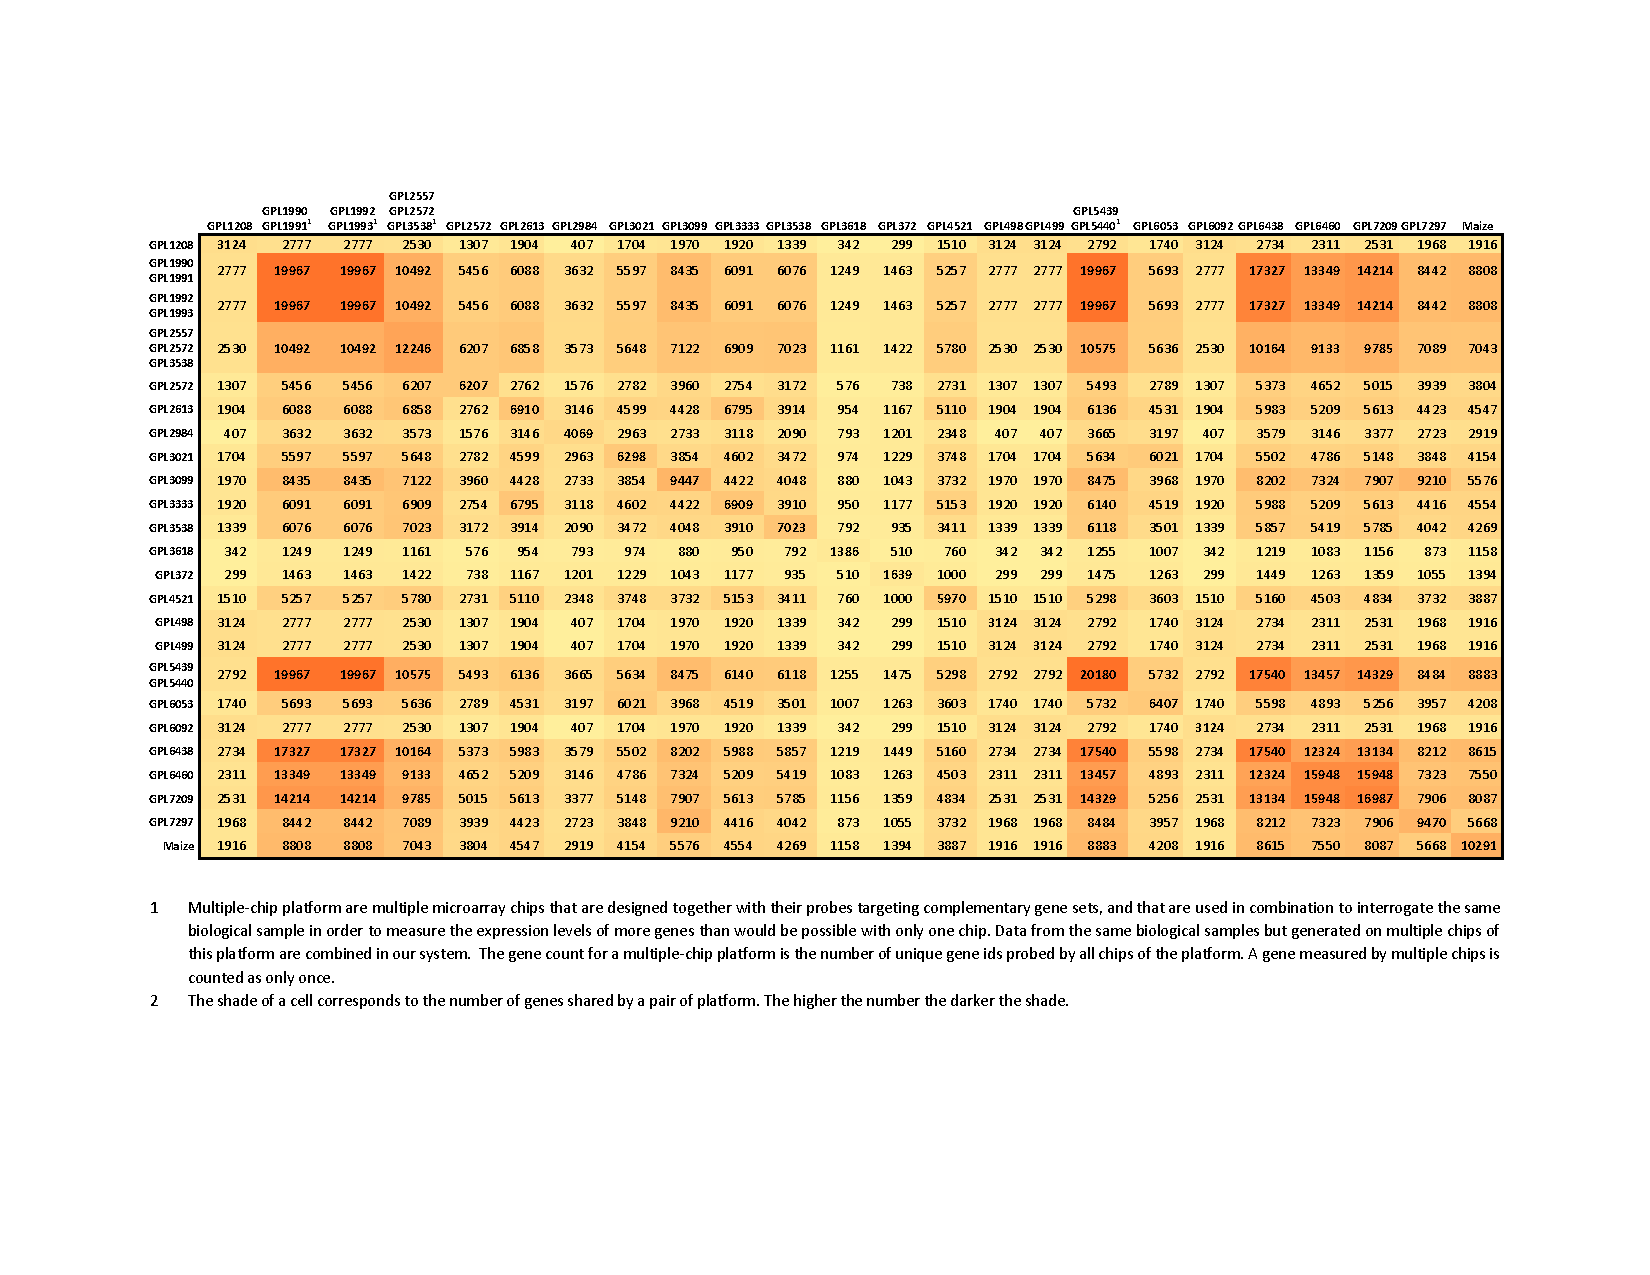
\includegraphics[trim=2cm 2cm 2cm 2cm, clip=true, width=1\textwidth] 	
		{ApdxB-overlap-TB.pdf} \\
	\end{tabular}
\end{sidewaystable}


\begin{figure}[t]
	\centering
	\caption{Gene platform coverage}\label{fig:maize-accu-platform-count}
	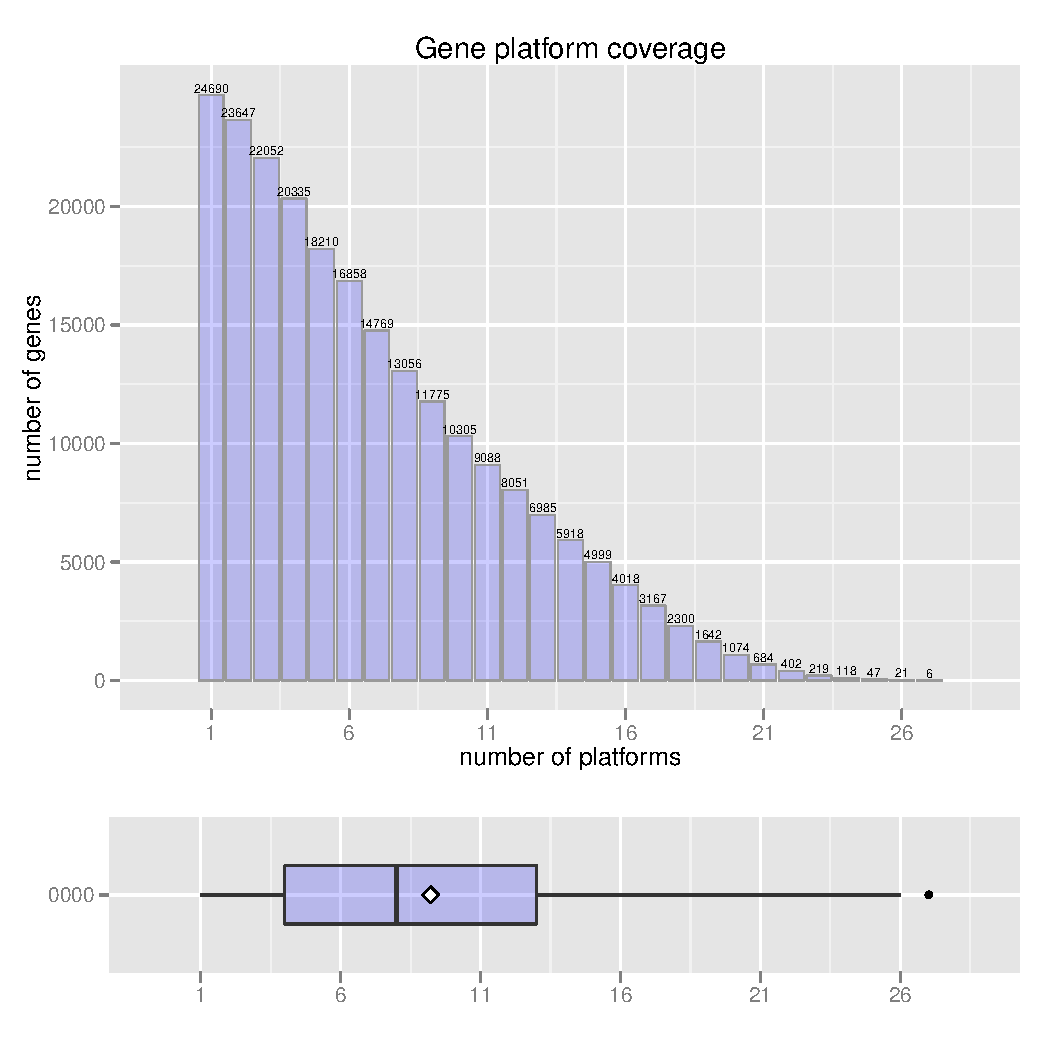
\includegraphics[trim=0cm 0cm 0cm 1.2cm, clip=true, 
		width=1\textwidth]{ApdxB-accu_platform_count.pdf}
	\caption*{The figures show gene platform coverage. Above, a bar chart 
	showing the number of genes (y-axis) covered by  at least x platforms 
	indicated by the x-axis. 
	The leftmost bar shows that each gene is measured on at least 1 
	platform, whereas there are only 6 genes that have been measured on all 27 
	platforms of the compendium (the rightmost bar). 
	The box plot below indicates the number of platforms a gene has been 
	measured on (gene centric and non-cumulative counting), showing that most 
	genes are measured on 4 to 13 platforms with an average of 9 (the diamond).}
\end{figure}


\begin{figure}[t]
	\centering
	\caption{Gene contrast coverage}\label{fig:maize-accu-contrast-count}
	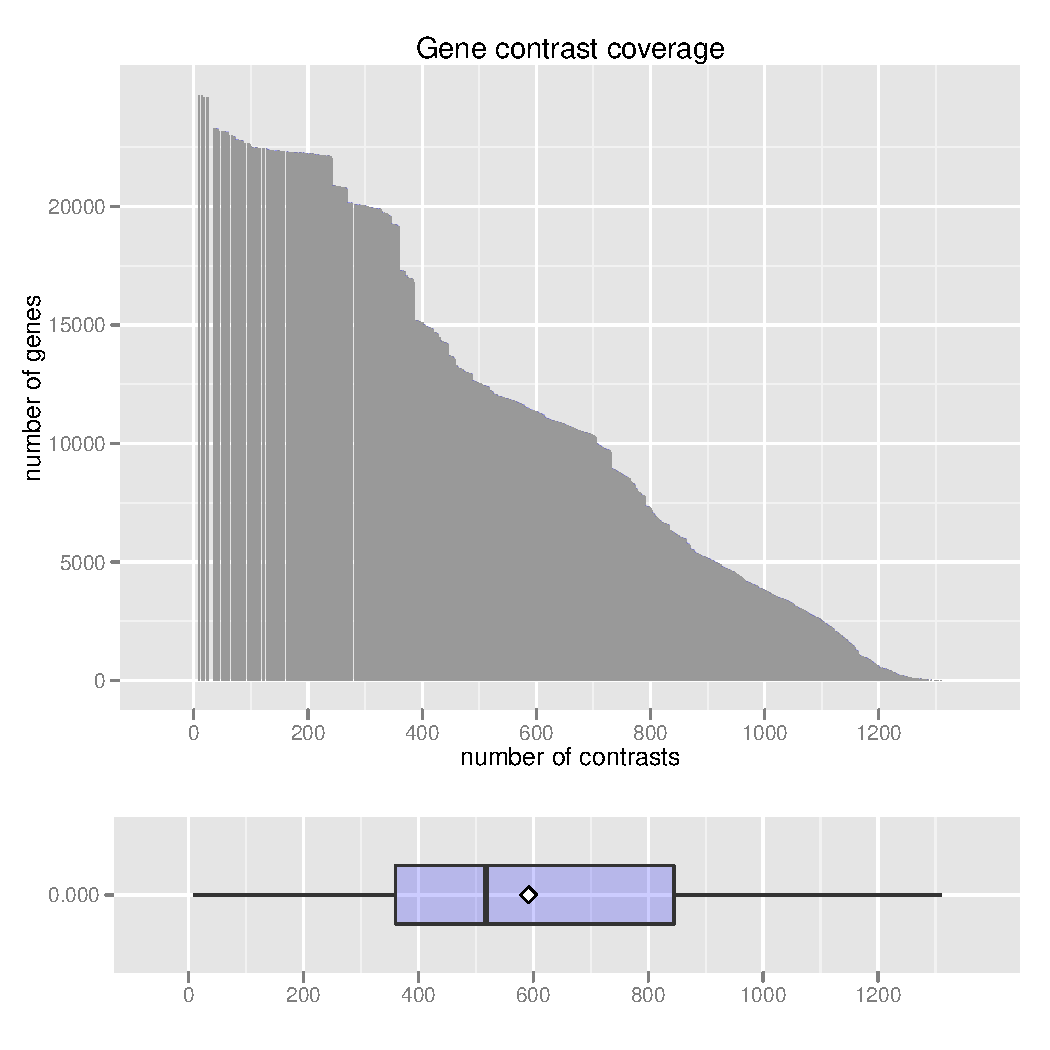
\includegraphics[trim=0cm 0cm 0cm 1.2cm, clip=true, 	 	
		width=1\textwidth]{ApdxB-accu_contrast_count.pdf}
	\caption*{The figures show gene contrast coverage. 
	Above, a bar chart showing the number of genes (y-axis) covered by at least 
	x contrasts indicated by the x-axis. 
	The leftmost bar shows that every gene has measurements in at least a small 
	number of contrasts (the corresponding x value of this bar is close to but 
	not at 0). 
	Few genes have measurements in all 1310 contrasts in the compendium (the 
	rightmost bar). 
	The box plot below indicates the number of contrasts a gene has been 
	measured in (gene centric and non-cumulative counting), showing that  most 
	genes have measurements in between 300 to 900 contrasts with an average of 
	592 (the diamond). }
\end{figure}

%%%%%%%%%%%%%%%%%%%%%%%%%%%%%%%%%%%%%%%%%%%%%%%%%%
% Keep the following \cleardoublepage at the end of this file, 
% otherwise \includeonly includes empty pages.
\cleardoublepage

% vim: tw=70 nocindent expandtab foldmethod=marker foldmarker={{{}{,}{}}}
